\section{Experimental}

We mix "equal" amounts of H$_2$O and D$_2$O and leave it overnight to produce roughly 1:2:1 ratio of H$_2$O:HOD:D$_2$O as roughly verified by the RGA. If we consider being a singular oxygen atom looking at a sea of H$_2$O and D$_2$O, it has a 1/4 probability of grabbing H or D twice. It then has a 1/2 chance of grabbing an H and D in either order, which gives us the 1:2:1 ratio.

To generalize this, we can write the fraction of H$_2$O in the sample to be $\gamma$ and the D$_2$O to be $1-\gamma$. The probabilities of yielding any combination is then found quickly:

\begin{align}
H_2O& = \gamma^2 \\
HOD& = 2\gamma(1-\gamma) \\
D_2O& = (1-\gamma)^2
\end{align}

For the sake of readability, let (H$_2$O, HOD, D$_2$O) be represented as (1, 2, 3) respectively.

\begin{figure}[H]
\label{fig: mixture}
\centering
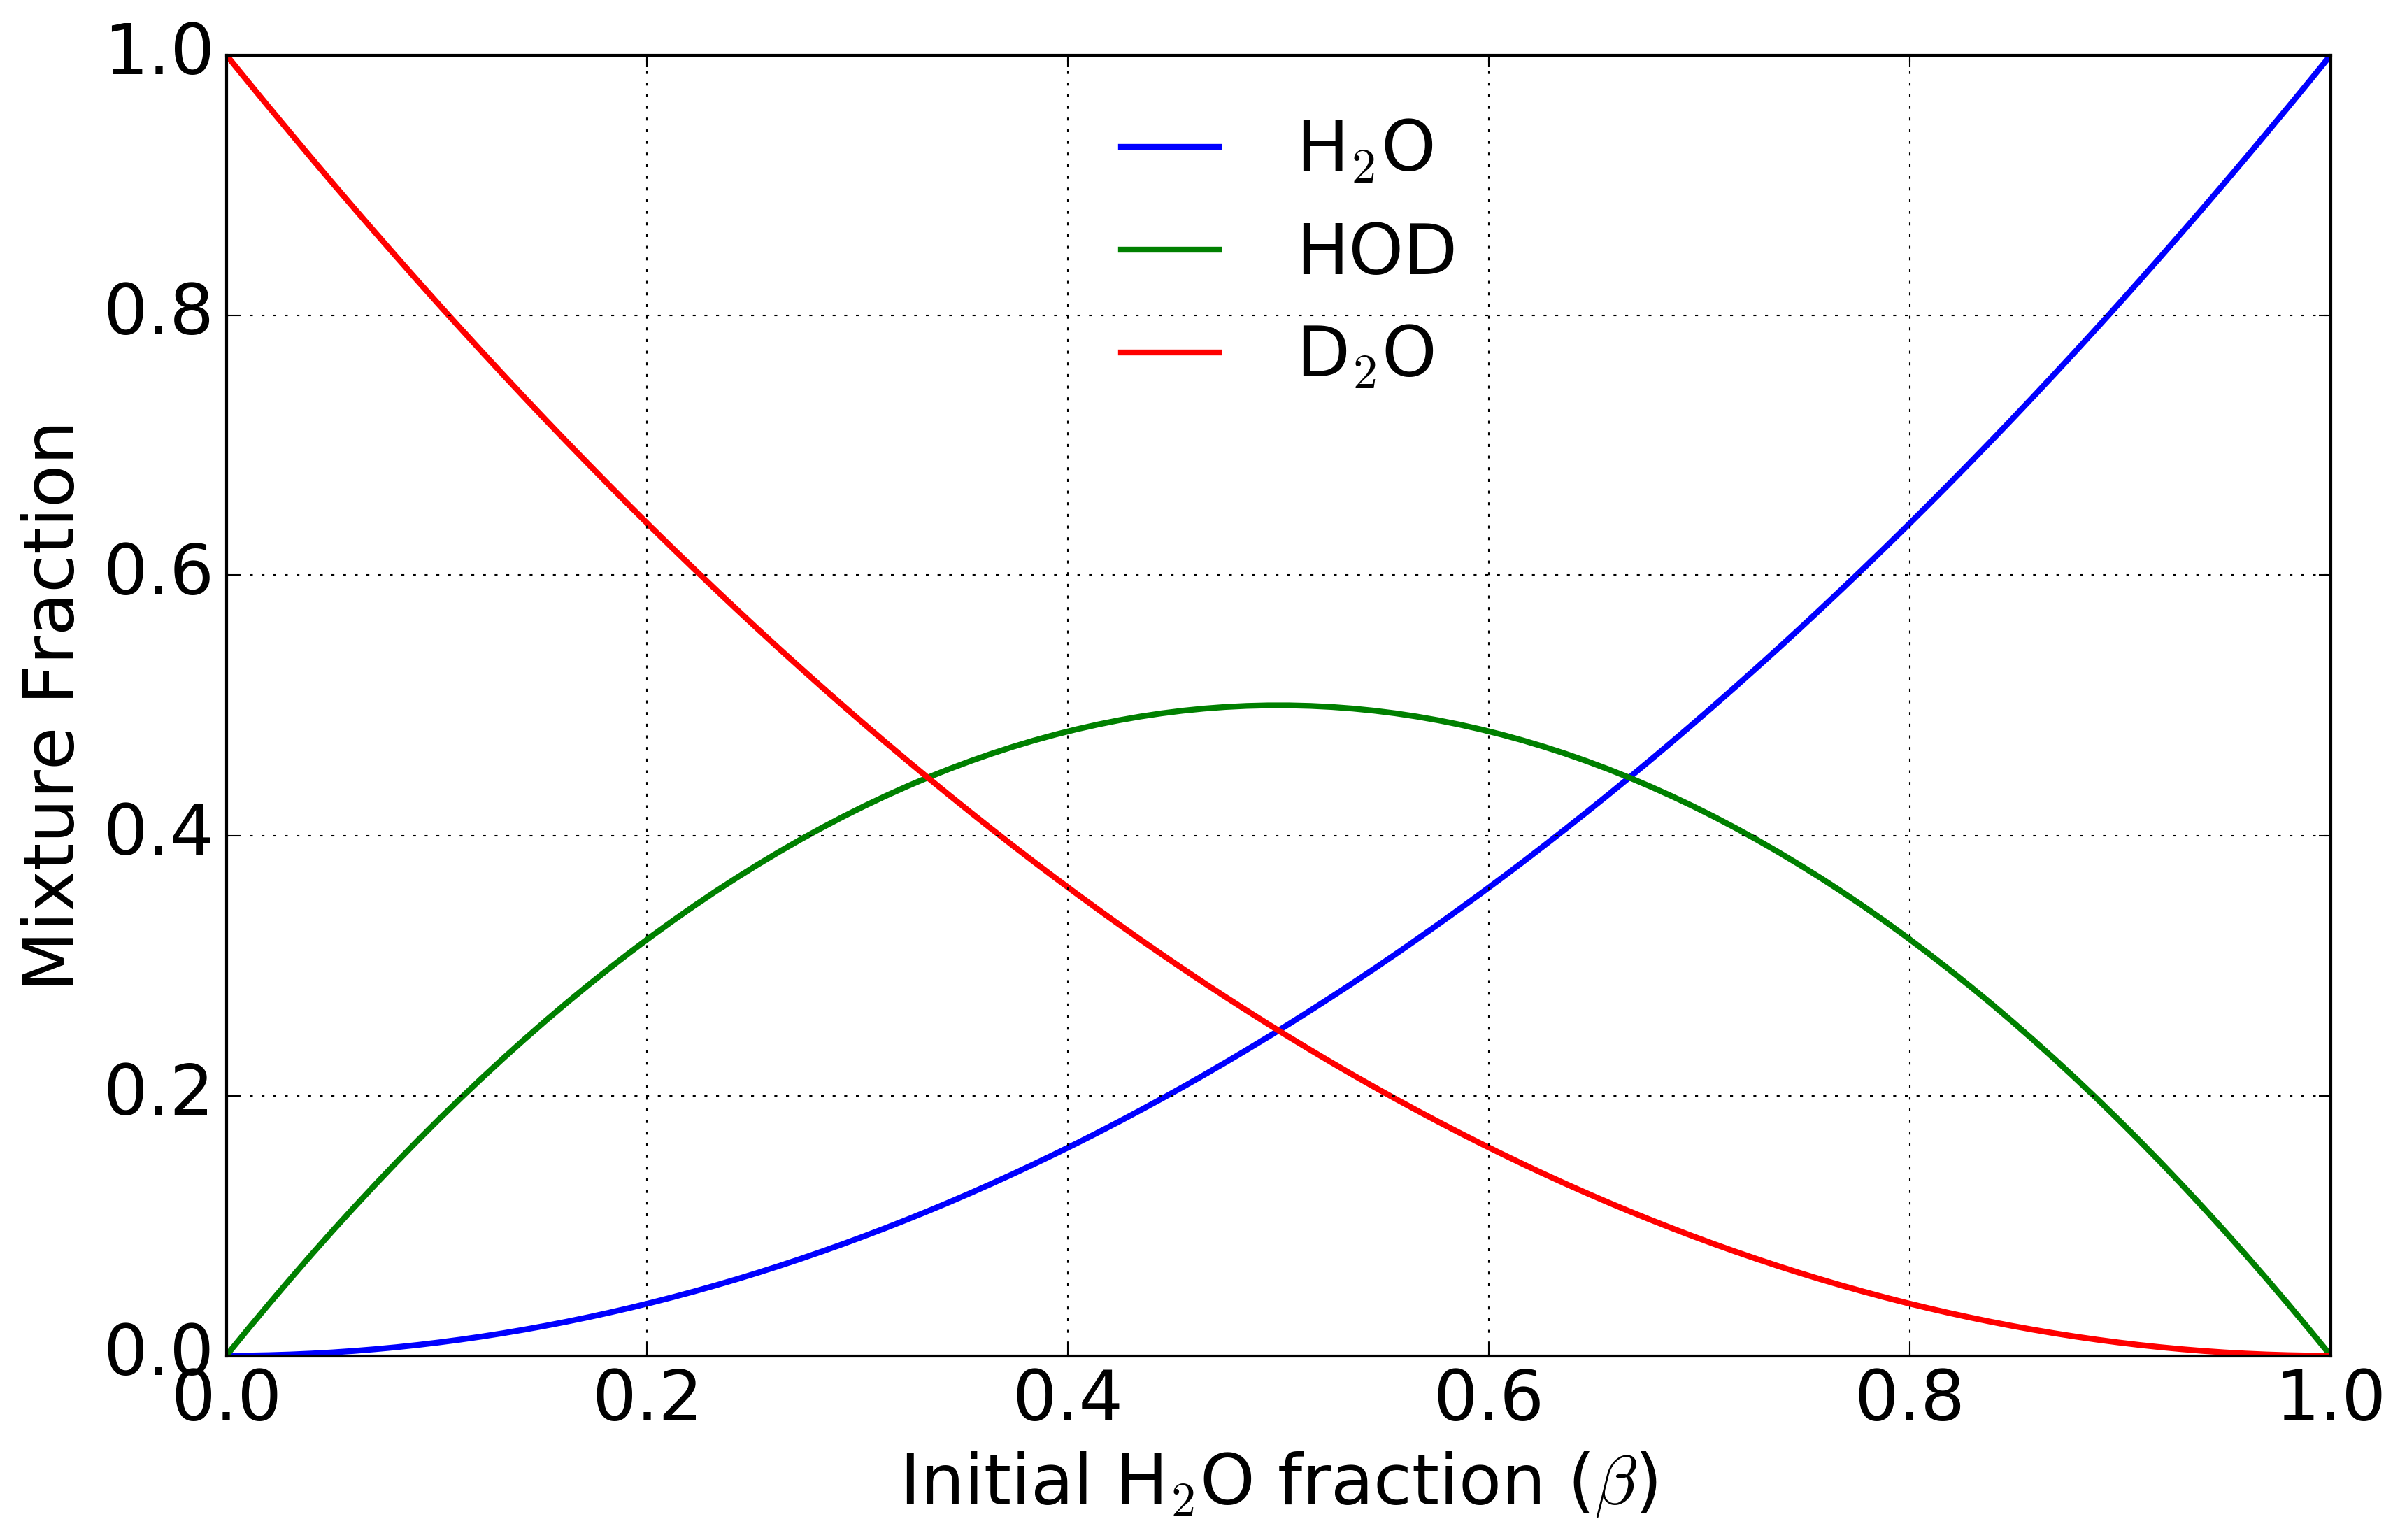
\includegraphics[width=0.8\textwidth]{images/behod_isotopologues.png}
\caption{}
\end{figure}

Reading water with an RGA causes some known fractionation, where the H$_2$O is broken into its constituents, including OH$^+$ and O$^+$. We expect then to see a lower mass 18 peak than normal, to truly know what the ratios are, we have to calibrate the RGA ourselves.

Possible fractionation pathways:

\begin{align}
P'_{18} = & \alpha P_{H_2O} + \beta (\frac{P_{HOD}}{2}+P_{D_2O}) \\
P'_{19} = & \alpha P_{HOD} \\
P'_{20} = & \alpha P_{D_2O} \\
P'_{17} = & \beta (\frac{P_{HOD}}{2} + P_{H_2O}) \\
P'_{16} = & \gamma (P_{H_2O} + P_{HOD} + P_{D_2O}) \\
1 = & \alpha + \beta + \gamma
\end{align}

By solving this system of equations, we get:

\begin{table}[H]
\centering
\begin{tabular}{l|l|l|l}
Date      & $\alpha$ & $\beta$  & $\gamma$ \\ \hline
8/20/2018 & 0.769 & 0.178 & 0.052 \\ \hline
8/21/2018 & 0.769 & 0.184 & 0.047 \\ \hline
8/22/2018 & 0.767 & 0.193 & 0.040
\end{tabular}
\end{table}

76.8\% of the real value as cited by the RGA program itself; this is also true for HOD and D$_2$O. Of that lost 23.2\%, 18.4\% goes to OH$^+$, but for the isotopogues of HOD and D$_2$O, we would need to consider which mass signal it will add to. No other mode of fractionation will contribute to the other water isotopologue peaks

\begin{align}
P'_1 & = \alpha P_1 + \beta P_3 + \frac{\beta}{2} P_2 \\
P'_2 & = \alpha P_2 \\
P'_3 & = \alpha P_3
\end{align}

Where we let $\alpha = 0.744$ and $\beta=0.256$ per the SRS RGA software. Where P is the real pressure accounting for fractionation, and P' is the raw observed pressure value. Solving for the real pressure, we find:

\begin{align}
P_1 & = \frac{1}{\alpha}\left(P'_1 - \frac{\beta}{\alpha}P'_3 - \frac{\beta}{2\alpha} P'_2\right) \\
P_2 & = \frac{P'_2}{\alpha} \\
P_3 & = \frac{P'_3}{\alpha}
\end{align}

\section{Be$^+$ + HOD branching ratio}

Now that we can characterize the pressures in the chamber more accurately, we then consider the possible reactions between the Be$^+$ and water isotopologues:

\begin{align}
Be^+ + H_2O & \rightarrow BeOH^+ + H \\
Be^+ + HOD & \rightarrow BeOH^+ + H \label{eq: beoh} \\
 & \rightarrow BeOD^+ + H \label{eq: beod} \\
Be^+ + D_2O & \rightarrow BeOD^+ + D
\end{align}

Which can then be written as a system of differential equations.

\begin{align}
\dot{Be}(t) & = -(k_1\rho_1+k_2\rho_2+k_3\rho_3)Be(t) \\
\dot{BeOH}(t) & = (k_1\rho_1+(1-\eta)k_2\rho_2)Be(t) \\
\dot{BeOD}(t) & = (k_3\rho_3+\eta k_2\rho_2)Be(t)
\end{align}

We are interested in reactions \ref{eq: beoh} and \ref{eq: beod} and the ratio between the two ($\eta$), which is not directly found from the ratio of the production rates of the two ions. Since this is a ratio, we don't need to concern ourselves with calculating the density ($\rho$), the RGA pressure is fine.

\begin{align}
\beta \equiv \frac{\dot{BeOD}}{\dot{BeOH}} & = \frac{k_3P_3 + \eta k_2P_2}{k_1P_1 + (1-\eta)k_2P_2} \\
\eta & = \frac{\beta(k_1P_1 + k_2P_2)-k_3P_3}{k_2P_2(1+\beta)}
\end{align}

The theorists found that the statistical value of the reaction is around 3, but with dynamics, tends towards $\frac{\eta}{1-\eta} = 1.7$ or $\eta=0.63$ for Be$^+$(S).